\documentclass[12pt,a4paper]{article}

% --- Page Layout -------------------------------------------------------------
\usepackage[a4paper, margin=0.8in, headheight=14pt]{geometry}

% --- Fonts (XeLaTeX) ---------------------------------------------------------
\usepackage{fontspec}
\usepackage{unicode-math}
\setmainfont{TeX Gyre Pagella}
\setmonofont[Scale=0.88]{TeX Gyre Cursor}
\setmathfont{Latin Modern Math}

% --- Packages ---------------------------------------------------------------
\usepackage{xcolor}
\usepackage{titlesec}
\usepackage{enumitem}
\usepackage{tabularx}
\usepackage{booktabs}
\usepackage{array}
\usepackage{amsmath}
\usepackage{tikz}
\usetikzlibrary{shapes.geometric, arrows.meta, positioning, calc, fit, decorations.pathreplacing}
\usepackage{tcolorbox}
\tcbuselibrary{skins, breakable}
\usepackage{hyperref}
\usepackage{fancyhdr}
\usepackage{graphicx}
\usepackage{microtype}
\hyphenpenalty=10000
\exhyphenpenalty=10000
\sloppy
\usepackage{caption}
\usepackage{setspace}
\usepackage{multirow}
\usepackage{tocloft}

% --- Q&A helper --------------------------------------------------------------
\newcommand{\Q}[1]{\textbf{#1}\par\noindent\ignorespaces}

% --- Colour Palette ----------------------------------------------------------
\definecolor{myred}{RGB}{196,30,58}
\definecolor{mydark}{RGB}{30,30,50}
\definecolor{mygreen}{RGB}{14,120,80}
\definecolor{myteal}{RGB}{0,130,140}
\definecolor{myamber}{RGB}{180,100,0}
\definecolor{mypurple}{RGB}{100,30,160}
\definecolor{mygray}{RGB}{246,247,249}
\definecolor{mgframe}{RGB}{180,185,200}
\definecolor{watermark}{RGB}{145,150,170}
\definecolor{hdrred}{RGB}{250,232,235}
\definecolor{hdrgreen}{RGB}{220,244,233}
\definecolor{hdrteal}{RGB}{220,242,244}
\definecolor{hdramber}{RGB}{253,242,215}
\definecolor{hdrpurple}{RGB}{238,228,255}

% --- Section Formatting ------------------------------------------------------
\titleformat{\section}
  {\large\bfseries\color{myred}}{\thesection.}{0.5em}{}
  [\vspace{1pt}{\color{myred}\rule{\linewidth}{0.8pt}}]
\titleformat{\subsection}
  {\normalsize\bfseries\color{myteal}}{\thesubsection}{0.5em}{}
\titlespacing*{\section}{0pt}{18pt}{7pt}
\titlespacing*{\subsection}{0pt}{11pt}{4pt}

% --- Paragraph ---------------------------------------------------------------
\setlength{\parindent}{0pt}
\setlength{\parskip}{4pt}

% --- TOC Styling -------------------------------------------------------------
\renewcommand{\cfttoctitlefont}{\large\bfseries\color{myred}}
\renewcommand{\cftaftertoctitle}{\par\noindent{\color{myred}\rule{\linewidth}{0.8pt}}}
\setlength{\cftbeforetoctitleskip}{0pt}
\setlength{\cftaftertoctitleskip}{6pt}
\renewcommand{\cftsecfont}{\normalsize\bfseries\color{mydark}}
\renewcommand{\cftsecpagefont}{\normalsize\bfseries\color{mydark}}
\renewcommand{\cftsecleader}{\cftdotfill{\cftdotsep}}
\setlength{\cftbeforesecskip}{7pt}
\renewcommand{\cftsubsecfont}{\small\color{mydark}}
\renewcommand{\cftsubsecpagefont}{\small\color{mydark}}
\setlength{\cftbeforesubsecskip}{3pt}
\setlength{\cftsubsecindent}{1.4em}

% --- Table helpers -----------------------------------------------------------
\renewcommand{\arraystretch}{1.45}
\setlength{\tabcolsep}{6pt}
\newcolumntype{B}[1]{>{\small\bfseries\raggedright\arraybackslash}m{#1}}
\newcolumntype{Y}{>{\small\raggedright\arraybackslash}X}
\renewcommand{\tabularxcolumn}[1]{m{#1}}

% --- Header / Footer ---------------------------------------------------------
\pagestyle{fancy}
\fancyhf{}
\fancyhead[L]{\small\color{myred}\textbf{BS-PH101}\;\color{mydark}--- Physics-I}
\fancyhead[R]{\small\color{myteal}\textbf{Module 3 Notes}}
\fancyfoot[C]{\small\color{mydark}\thepage}
\fancyfoot[R]{\small\color{watermark}\textit{\copyright\ Biraj}}
\renewcommand{\headrulewidth}{0.5pt}
\renewcommand{\footrulewidth}{0.3pt}

% --- Hyperref ---------------------------------------------------------------
\hypersetup{
  colorlinks=true, linkcolor=myteal, urlcolor=myteal,
  pdfauthor={Biraj Sarkar},
  pdftitle={BS-PH101 --- Module 3 Notes}
}

% --- tcolorbox styles --------------------------------------------------------
\tcbset{
  tikzbox/.style={
    colback=mygray, colframe=mgframe, boxrule=0.6pt, arc=4pt,
    left=8pt, right=8pt, top=6pt, bottom=6pt,
    colbacktitle=mgframe, coltitle=mydark, fonttitle=\small\bfseries
  },
  defbox/.style={
    colback=hdrgreen, colframe=mygreen, boxrule=0.8pt, arc=4pt,
    left=9pt, right=9pt, top=6pt, bottom=6pt,
    colbacktitle=mygreen, coltitle=white, fonttitle=\small\bfseries
  },
  formulabox/.style={
    colback=hdrteal, colframe=myteal, boxrule=0.8pt, arc=4pt,
    left=9pt, right=9pt, top=7pt, bottom=7pt,
    colbacktitle=myteal, coltitle=white, fonttitle=\small\bfseries
  },
  examplebox/.style={
    colback=hdramber, colframe=myamber, boxrule=0.8pt, arc=4pt,
    left=9pt, right=9pt, top=6pt, bottom=6pt,
    colbacktitle=myamber, coltitle=white, fonttitle=\small\bfseries
  },
  masonbox/.style={
    colback=hdrpurple, colframe=mypurple, boxrule=0.8pt, arc=4pt,
    left=9pt, right=9pt, top=6pt, bottom=6pt,
    colbacktitle=mypurple, coltitle=white, fonttitle=\small\bfseries
  },
  exambox/.style={
    colback=hdrpurple, colframe=mypurple, boxrule=1pt, arc=5pt,
    left=10pt, right=10pt, top=8pt, bottom=8pt,
    colbacktitle=mypurple, coltitle=white, fonttitle=\bfseries,
    breakable, title after break={\textbf{Frequently Asked / Viva Questions (contd.)}}
  }
}
\tcbset{breakable}

% --- TikZ Styles -------------------------------------------------------------
\tikzset{
  block/.style={rectangle, draw=myteal, fill=hdrteal, text width=2.4cm, align=center, minimum height=0.95cm, font=\small, rounded corners=3pt, line width=0.7pt},
  redblock/.style={rectangle, draw=myred, fill=hdrred, text width=2.4cm, align=center, minimum height=0.95cm, font=\small, rounded corners=3pt, line width=0.7pt},
  arrow/.style={-Stealth, thick, color=mydark},
  redarrow/.style={-Stealth, thick, color=myred},
  line/.style={thick, color=mydark}
}

\begin{document}

% --- Title Page --------------------------------------------------------------
\begin{center}
  {\LARGE\bfseries\color{myred} BS-PH101 --- Physics-I}\\[5pt]
  {\normalsize\color{mydark} Semester I/II \quad$\bullet$\quad 3L:1T:0P \quad$\bullet$\quad 4 Credits}\\[3pt]
  {\normalsize\color{myteal}\textbf{Module 3 Comprehensive Exam Notes: Electromagnetism \& Materials}}\\[3pt]
  {\small\color{mydark} CGEC \;$|$\; B.Tech ECE (2023--27) \;$|$\; \textit{Biraj Sarkar}}
\end{center}
\vspace{2pt}
\noindent{\color{myred}\rule{\linewidth}{1.5pt}}
\vspace{2pt}
\hypersetup{linkcolor=mydark}
\tableofcontents
\hypersetup{linkcolor=myteal}
\newpage

% =============================================================================
% SECTION 1: MAXWELL'S EQUATIONS & EM WAVES
% =============================================================================
\section{Maxwell's Equations and Electromagnetic Waves}

\subsection{Maxwell's Four Fundamental Equations}

Maxwell unified electricity and magnetism into four differential and integral equations governing electromagnetic phenomena.

\begin{tcolorbox}[formulabox, title={\textbf{Maxwell's Equations in Differential and Integral Forms}}]
\begin{enumerate}[leftmargin=*, itemsep=4pt]
  \item \textbf{Gauss's Law for Electrostatics:} Net electric flux through a closed surface equals charge enclosed:
  \begin{equation}
  \nabla \cdot \vec{D} = \rho \iff \oint_S \vec{D} \cdot d\vec{A} = Q_{\text{enclosed}} \quad (\vec{D} = \epsilon_0 \vec{E} + \vec{P})
  \end{equation}
  \item \textbf{Gauss's Law for Magnetostatics:} Magnetic monopoles do not exist (magnetic flux lines are continuous loops):
  \begin{equation}
  \nabla \cdot \vec{B} = 0 \iff \oint_S \vec{B} \cdot d\vec{A} = 0
  \end{equation}
  \item \textbf{Faraday's Law of Electromagnetic Induction:} Time-varying magnetic field produces an electric field:
  \begin{equation}
  \nabla \times \vec{E} = -\frac{\partial \vec{B}}{\partial t} \iff \oint_C \vec{E} \cdot d\vec{r} = -\frac{\partial}{\partial t}\int_S \vec{B} \cdot d\vec{A}
  \end{equation}
  \item \textbf{Ampere-Maxwell Law:} Magnetic fields are generated by electric currents and time-varying electric fields:
  \begin{equation}
  \nabla \times \vec{H} = \vec{J} + \frac{\partial \vec{D}}{\partial t} \iff \oint_C \vec{H} \cdot d\vec{r} = \int_S \left(\vec{J} + \frac{\partial \vec{D}}{\partial t}\right) \cdot d\vec{A}
  \end{equation}
\end{enumerate}
\end{tcolorbox}

\subsection{Displacement Current and Wave Equation in Free Space}

Maxwell modified Ampere's law ($\nabla \times \vec{H} = \vec{J}$) by taking the divergence of both sides. Since $\nabla \cdot (\nabla \times \vec{H}) = 0$, it required $\nabla \cdot \vec{J} = 0$, which violates the charge continuity equation $\nabla \cdot \vec{J} + \frac{\partial \rho}{\partial t} = 0$ for time-varying fields.

Substituting $\rho = \nabla \cdot \vec{D}$ into continuity equation:
\begin{equation}
\nabla \cdot \vec{J} + \frac{\partial}{\partial t}(\nabla \cdot \vec{D}) = 0 \implies \nabla \cdot \left( \vec{J} + \frac{\partial \vec{D}}{\partial t} \right) = 0
\end{equation}
Thus, Maxwell introduced the \textbf{Displacement Current Density} $\vec{J}_d = \frac{\partial \vec{D}}{\partial t} = \epsilon_0 \frac{\partial \vec{E}}{\partial t}$.

\begin{tcolorbox}[formulabox, title={\textbf{Electromagnetic Wave Equation and Speed of Light}}]
In free space ($\rho = 0, \vec{J} = 0, \mu = \mu_0, \epsilon = \epsilon_0$), taking curl of Faraday's law yields:
\begin{equation}
\nabla \times (\nabla \times \vec{E}) = -\frac{\partial}{\partial t}(\nabla \times \vec{B}) \implies \nabla(\nabla \cdot \vec{E}) - \nabla^2 \vec{E} = -\mu_0 \epsilon_0 \frac{\partial^2 \vec{E}}{\partial t^2}
\end{equation}
Since $\nabla \cdot \vec{E} = 0$, this simplifies to the standard 3D wave equation:
\begin{equation}
\nabla^2 \vec{E} = \mu_0 \epsilon_0 \frac{\partial^2 \vec{E}}{\partial t^2} \quad \text{and} \quad \nabla^2 \vec{B} = \mu_0 \epsilon_0 \frac{\partial^2 \vec{B}}{\partial t^2}
\end{equation}
Comparing with $\nabla^2 \psi = \frac{1}{v^2}\frac{\partial^2\psi}{\partial t^2}$, the wave velocity in vacuum is:
\begin{equation}
c = \frac{1}{\sqrt{\mu_0 \epsilon_0}} = \frac{1}{\sqrt{(4\pi \times 10^{-7}) (8.854 \times 10^{-12})}} = 2.998 \times 10^8 \text{ m/s}
\end{equation}
\end{tcolorbox}

\subsection{Poynting Vector and Energy Flow}

\begin{tcolorbox}[defbox, title={\textbf{Definition: Poynting Vector}}]
The \textbf{Poynting Vector ($\vec{S}$)} represents the directional energy flux density (rate of energy transfer per unit area) of an electromagnetic field:
\begin{equation}
\vec{S} = \vec{E} \times \vec{H} \quad \left(\text{in } \frac{\text{W}}{\text{m}^2}\right)
\end{equation}
The time-averaged Poynting vector intensity for a plane wave is $I = \langle S \rangle = \frac{1}{2} c \epsilon_0 E_0^2$.
\end{tcolorbox}

\begin{tcolorbox}[examplebox, title={\textbf{Solved Problem 1: Displacement Current in a Capacitor}}]
\textbf{Problem:} A parallel-plate capacitor with circular plates of radius $R = 0.1\text{ m}$ is being charged by a current $I = 2.0\text{ A}$. Calculate: (a) Displacement current $I_d$, (b) Rate of change of electric field $dE/dt$.

\textbf{Solution:}\par\noindent
\begin{enumerate}[leftmargin=*, itemsep=2pt]
  \item Total displacement current between plates equals conduction current in wires: $\mathbf{I_d = 2.0\text{ A}}$.
  \item Plate area $A = \pi R^2 = \pi (0.1)^2 = 0.0314\text{ m}^2$.
  \item $I_d = \epsilon_0 A \frac{dE}{dt} \implies \frac{dE}{dt} = \frac{I_d}{\epsilon_0 A}$:
   \begin{equation}
   \frac{dE}{dt} = \frac{2.0}{(8.854 \times 10^{-12}) \times 0.0314} = \mathbf{7.19 \times 10^{11}\text{ V/(m}\cdot\text{s)}}
   \end{equation}
\end{enumerate}
\end{tcolorbox}

% =============================================================================
% SECTION 2: DIELECTRIC PROPERTIES OF MATERIALS
% =============================================================================
\section{Dielectric Properties of Materials}

\subsection{Dielectric Vectors: Polarisation, Susceptibility, Permittivity}

Dielectrics are electrical insulators that can be polarized by an applied electric field.

\begin{tcolorbox}[formulabox, title={\textbf{Fundamental Dielectric Relations}}]
\begin{itemize}[leftmargin=*, itemsep=3pt]
  \item \textbf{Electric Dipole Moment ($\vec{p}$):} $\vec{p} = q \vec{d}$ (directed from $-q$ to $+q$).
  \item \textbf{Polarisation Vector ($\vec{P}$):} Dipole moment per unit volume: $\vec{P} = N \vec{p}$.
  \item \textbf{Electric Displacement ($\vec{D}$):}
  \begin{equation}
  \vec{D} = \epsilon_0 \vec{E} + \vec{P} = \epsilon_0 \epsilon_r \vec{E}
  \end{equation}
  \item \textbf{Electric Susceptibility ($\chi_e$):} $\vec{P} = \epsilon_0 \chi_e \vec{E} \implies \epsilon_r = 1 + \chi_e$.
\end{itemize}
\end{tcolorbox}

\textbf{Microscopic Polarisation Mechanisms:}\par\vspace{6pt}\noindent
\begin{tabularx}{\linewidth}{|B{3.2cm}|Y|Y|}
\hline
\textbf{Mechanism} & \textbf{Origin / Description} & \textbf{Temperature Dependence} \\
\hline
\textbf{Electronic ($\alpha_e$)} & Displacement of electron cloud relative to nucleus in an atom. & Independent of temperature ($T$). \\
\hline
\textbf{Ionic ($\alpha_i$)} & Relative displacement of positive and negative ions in a crystal lattice. & Independent of temperature ($T$). \\
\hline
\textbf{Orientational ($\alpha_o$)} & Realignment of permanent molecular dipoles along external field. & Strongly temperature dependent ($\alpha_o \propto 1/T$). \\
\hline
\textbf{Space-Charge ($\alpha_s$)} & Accumulation of free charge carriers at interfaces/grain boundaries. & Dependent on temperature and frequency. \\
\hline
\end{tabularx}

\subsection{Clausius-Mossotti Equation}

Consider a solid dielectric where local field acting on an atom is the \textbf{Lorentz Field}:
\begin{equation}
E_{\text{local}} = E + \frac{P}{3\epsilon_0}
\end{equation}
The induced dipole moment per atom is $p = \alpha E_{\text{local}}$, so total polarisation for $N$ atoms per unit volume is:
\begin{equation}
P = N p = N \alpha E_{\text{local}} = N \alpha \left( E + \frac{P}{3\epsilon_0} \right)
\end{equation}

\begin{tcolorbox}[formulabox, title={\textbf{Clausius-Mossotti Relation Derivation}}]
Solving for $P$:
\begin{equation}
P \left( 1 - \frac{N \alpha}{3\epsilon_0} \right) = N \alpha E \implies P = \frac{N \alpha E}{1 - \frac{N \alpha}{3\epsilon_0}}
\end{equation}
Since $P = (\epsilon_r - 1)\epsilon_0 E$, substitute for $P$:
\begin{equation}
(\epsilon_r - 1)\epsilon_0 E = \frac{N \alpha E}{1 - \frac{N \alpha}{3\epsilon_0}} \implies \frac{\epsilon_r - 1}{\epsilon_r + 2} = \frac{N \alpha}{3 \epsilon_0}
\end{equation}
This connects the macroscopic dielectric constant $\epsilon_r$ with the microscopic atomic polarizability $\alpha$.
\end{tcolorbox}

% =============================================================================
% SECTION 3: MAGNETIC PROPERTIES OF MATERIALS
% =============================================================================
\section{Magnetic Properties of Materials}

\subsection{Magnetic Vectors and Classification}

\begin{tcolorbox}[formulabox, title={\textbf{Magnetic Field Relations}}]
\begin{itemize}[leftmargin=*, itemsep=3pt]
  \item \textbf{Magnetisation ($\vec{M}$):} Magnetic dipole moment per unit volume: $\vec{M} = \frac{\sum \vec{m}}{V}$.
  \item \textbf{Magnetic Flux Density ($\vec{B}$):} $\vec{B} = \mu_0 (\vec{H} + \vec{M}) = \mu_0 \mu_r \vec{H}$.
  \item \textbf{Magnetic Susceptibility ($\chi_m$):} $\vec{M} = \chi_m \vec{H} \implies \mu_r = 1 + \chi_m$.
\end{itemize}
\end{tcolorbox}

\textbf{Classification of Magnetic Materials:}\par\vspace{6pt}\noindent
\begin{tabularx}{\linewidth}{|B{3.0cm}|Y|Y|Y|}
\hline
\textbf{Property} & \textbf{Diamagnetic} & \textbf{Paramagnetic} & \textbf{Ferromagnetic} \\
\hline
\textbf{Atomic Dipoles} & No permanent dipoles. & Permanent dipoles present (random). & Permanent dipoles strongly aligned in domains. \\
\hline
\textbf{Susceptibility $\chi_m$} & Small and negative ($\sim -10^{-5}$). & Small and positive ($\sim 10^{-4}$). & Very large and positive ($\sim 10^3 - 10^5$). \\
\hline
\textbf{Permittivity $\mu_r$} & $\mu_r < 1$ slightly. & $\mu_r > 1$ slightly. & $\mu_r \gg 1$. \\
\hline
\textbf{Temp. Dependence} & Independent of $T$. & Curie Law ($\chi \propto 1/T$). & Curie-Weiss Law ($\chi \propto \frac{1}{T - T_c}$). \\
\hline
\textbf{External Field} & Repelled by magnetic fields. & Feebly attracted to magnetic fields. & Strongly attracted into magnetic fields. \\
\hline
\textbf{Examples} & Bismuth, Copper, Water, Gold. & Aluminium, Platinum, Oxygen. & Iron, Cobalt, Nickel, Gadolinium. \\
\hline
\end{tabularx}

\subsection{Hysteresis Loop (B-H Curve)}

\begin{tcolorbox}[tikzbox, title={Ferromagnetic Hysteresis (B-H) Loop}]
\centering
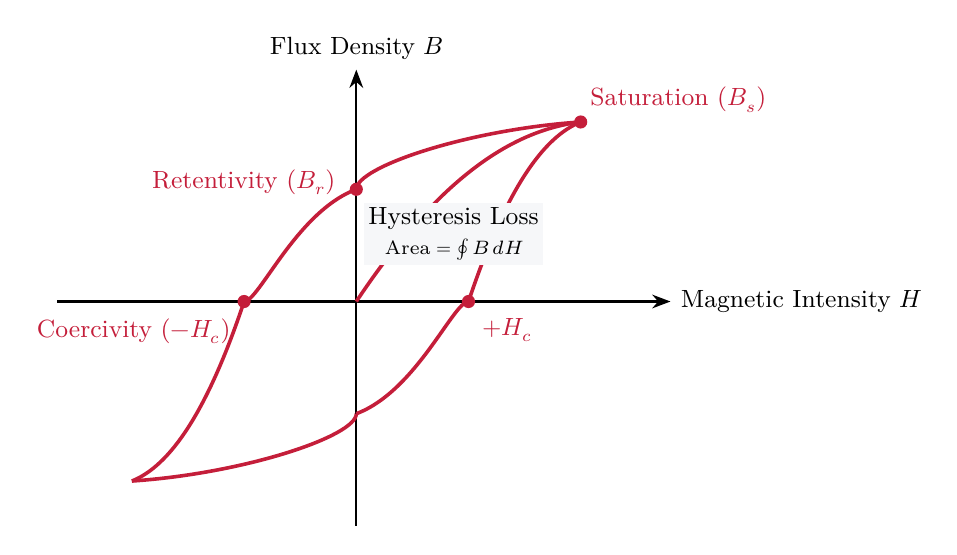
\begin{tikzpicture}[scale=0.95]
  % Axes
  \draw[-Stealth, thick] (-4,0) -- (4.2,0) node[right] {\small Magnetic Intensity $H$};
  \draw[-Stealth, thick] (0,-3) -- (0,3.1) node[above] {\small Flux Density $B$};
  
  % Hysteresis Loop
  \draw[myred, line width=1.3pt] (0,0) .. controls (1.2,1.8) and (2.2,2.3) .. (3,2.4);
  \draw[myred, line width=1.3pt] (3,2.4) .. controls (1.5,2.3) and (0,1.8) .. (0,1.5);
  \draw[myred, line width=1.3pt] (0,1.5) .. controls (-0.8,1.2) and (-1.3,0) .. (-1.5,0);
  \draw[myred, line width=1.3pt] (-1.5,0) .. controls (-2.0,-1.5) and (-2.5,-2.2) .. (-3,-2.4);
  \draw[myred, line width=1.3pt] (-3,-2.4) .. controls (-1.5,-2.3) and (0,-1.8) .. (0,-1.5);
  \draw[myred, line width=1.3pt] (0,-1.5) .. controls (0.8,-1.2) and (1.3,0) .. (1.5,0);
  \draw[myred, line width=1.3pt] (1.5,0) .. controls (2.0,1.5) and (2.5,2.2) .. (3,2.4);

  % Key Feature Markers & Labels
  \fill[myred] (3,2.4) circle (2.5pt);
  \node[myred, anchor=south west] at (3.0, 2.4) {\small Saturation ($B_s$)};

  \fill[myred] (0,1.5) circle (2.5pt);
  \node[myred, anchor=east] at (-0.15, 1.6) {\small Retentivity ($B_r$)};

  \fill[myred] (-1.5,0) circle (2.5pt);
  \node[myred, anchor=north east] at (-1.55, -0.1) {\small Coercivity ($-H_c$)};

  \fill[myred] (1.5,0) circle (2.5pt);
  \node[myred, anchor=north west] at (1.55, -0.1) {\small $+H_c$};

  % Hysteresis Loss text in clear region
  \node[align=center, fill=mygray, inner sep=1.5pt] at (1.3, 0.9) {\small Hysteresis Loss\\[-1pt]\scriptsize $\text{Area} = \oint B \, dH$};
\end{tikzpicture}
\end{tcolorbox}

\begin{tcolorbox}[defbox, title={\textbf{Hysteresis Terminology}}]
\begin{itemize}[leftmargin=*, itemsep=2pt]
  \item \textbf{Retentivity (Remanence $B_r$):} Residual flux density remaining in material when magnetising field $H$ is reduced to zero.
  \item \textbf{Coercivity ($H_c$):} Reverse magnetising field required to reduce residual flux density $B$ to zero.
  \item \textbf{Hysteresis Loss:} Energy dissipated per unit volume per cycle as heat during magnetisation reversal, equal to area enclosed by $B$-$H$ loop: $W_{\text{loss}} = \oint B \, dH$.
\end{itemize}
\end{tcolorbox}

\textbf{Soft vs. Hard Magnetic Materials:}\par\vspace{6pt}\noindent
\begin{tabularx}{\linewidth}{|B{3.2cm}|Y|Y|}
\hline
\textbf{Feature} & \textbf{Soft Magnetic Materials} & \textbf{Hard Magnetic Materials} \\
\hline
\textbf{Hysteresis Area} & Thin and narrow loop (low energy loss). & Broad and wide loop (high energy loss). \\
\hline
\textbf{Coercivity} & Very low coercivity ($H_c$ small). & Very high coercivity ($H_c$ large). \\
\hline
\textbf{Retentivity} & High retentivity, easily demagnetised. & High retentivity, retains magnetisation. \\
\hline
\textbf{Applications} & Transformer cores, electromagnets, inductors. & Permanent magnets, magnetic recording tapes, loudspeakers. \\
\hline
\end{tabularx}

\begin{tcolorbox}[examplebox, title={\textbf{Solved Problem 2: Hysteresis Loss Power Dissipation}}]
\textbf{Problem:} An iron ring of volume $V = 100\text{ cm}^3$ is subjected to a $50\text{ Hz}$ alternating magnetic field. If the area of the hysteresis loop corresponds to $250\text{ J/m}^3$ per cycle, calculate the power loss in watts.

\textbf{Solution:}\par\noindent
\begin{enumerate}[leftmargin=*, itemsep=2pt]
  \item Volume $V = 100 \times 10^{-6}\text{ m}^3 = 10^{-4}\text{ m}^3$.
  \item Frequency $f = 50\text{ Hz}$ (50 cycles/second).
  \item Energy loss per second (Power $P$) = Energy/cycle/volume $\times$ Volume $\times$ Frequency:
   \begin{equation}
   P = W_{\text{loss}} \times V \times f = 250\text{ J/m}^3 \times 10^{-4}\text{ m}^3 \times 50\text{ s}^{-1} = \mathbf{1.25\text{ W}}
   \end{equation}
\end{enumerate}
\end{tcolorbox}

% =============================================================================
% QUICK REVISION PAGE
% =============================================================================
\newpage
\begin{center}
  {\large\bfseries\color{myred} Quick Revision --- Module 3}\\[3pt]
  {\small\color{mydark} Electromagnetism \& Materials $|$ BS-PH101}
\end{center}
\noindent{\color{myred}\rule{\linewidth}{1.2pt}}
\vspace{4pt}

\begin{tcolorbox}[formulabox, title={\textbf{Key Formulas and Metrics at a Glance}}]
\renewcommand{\arraystretch}{1.35}
\begin{tabularx}{\linewidth}{B{5.0cm} X}
Maxwell 1 (Gauss Electro) & $\nabla \cdot \vec{D} = \rho \iff \oint_S \vec{D} \cdot d\vec{A} = Q_{\text{enclosed}}$ \\[4pt]
Maxwell 2 (Gauss Magneto) & $\nabla \cdot \vec{B} = 0 \iff \oint_S \vec{B} \cdot d\vec{A} = 0$ \\[4pt]
Maxwell 3 (Faraday) & $\nabla \times \vec{E} = -\frac{\partial \vec{B}}{\partial t} \iff \oint_C \vec{E} \cdot d\vec{r} = -\frac{\partial\Phi_B}{\partial t}$ \\[4pt]
Maxwell 4 (Ampere-Maxwell) & $\nabla \times \vec{H} = \vec{J} + \frac{\partial \vec{D}}{\partial t}$ \\[4pt]
Displacement Current & $\vec{J}_d = \frac{\partial \vec{D}}{\partial t} = \epsilon_0 \frac{\partial \vec{E}}{\partial t}$ \\[4pt]
Speed of Light in Vacuum & $c = \frac{1}{\sqrt{\mu_0 \epsilon_0}} = 3 \times 10^8\text{ m/s}$ \\[4pt]
Poynting Vector & $\vec{S} = \vec{E} \times \vec{H} \quad (\text{W/m}^2)$ \\[4pt]
Clausius-Mossotti Eq. & $\frac{\epsilon_r - 1}{\epsilon_r + 2} = \frac{N \alpha}{3 \epsilon_0}$ \\[4pt]
Magnetic Relations & $\vec{B} = \mu_0(\vec{H} + \vec{M})$ \quad and \quad $\mu_r = 1 + \chi_m$ \\[4pt]
Hysteresis Power Loss & $P_{\text{loss}} = (\oint B dH) \times \text{Volume} \times \text{Frequency}$ \\[4pt]
\end{tabularx}
\end{tcolorbox}

\begin{tcolorbox}[defbox, title={\textbf{One-Line Definitions}}]
\begin{itemize}[leftmargin=*, itemsep=2pt]
  \item \textbf{Displacement Current:} A quantity appearing in Maxwell's equations defined by rate of change of electric displacement field ($\vec{J}_d = \partial\vec{D}/\partial t$).
  \item \textbf{Poynting Vector:} A vector representing the directional energy flux density of an electromagnetic field ($\vec{S} = \vec{E} \times \vec{H}$).
  \item \textbf{Lorentz Local Field:} The actual local electric field acting at the position of an individual atom in a solid ($E_{\text{local}} = E + P/3\epsilon_0$).
  \item \textbf{Retentivity ($B_r$):} Residual magnetic flux density remaining in a ferromagnetic material when magnetising field $H$ is reduced to zero.
  \item \textbf{Coercivity ($H_c$):} The magnitude of reverse magnetic field intensity required to reduce residual magnetisation to zero.
\end{itemize}
\end{tcolorbox}

\begin{tcolorbox}[exambox, title={\textbf{Frequently Asked / Viva Questions}}]
\begin{enumerate}[topsep=0pt, label=\textbf{Q\arabic*.}, itemsep=5pt]
  \item \Q{Why did Maxwell modify Ampere's law and what term did he add?}
  Ampere's law ($\nabla \times \vec{H} = \vec{J}$) violated charge conservation for time-varying fields ($\nabla \cdot \vec{J} \neq 0$). Maxwell added displacement current density $\vec{J}_d = \partial\vec{D}/\partial t$.

  \item \Q{What is the physical significance of $\nabla \cdot \vec{B} = 0$?}
  It signifies that isolated magnetic monopoles do not exist in nature and magnetic flux lines always form continuous closed loops.

  \item \Q{What is Poynting vector and state its SI unit?}
  $\vec{S} = \vec{E} \times \vec{H}$ represents the rate of electromagnetic energy flow per unit area. Its SI unit is $\text{W/m}^2$.

  \item \Q{State the relation between dielectric constant $\epsilon_r$ and electric susceptibility $\chi_e$.}
  $\vec{D} = \epsilon_0 \vec{E} + \vec{P} = \epsilon_0(1 + \chi_e)\vec{E} = \epsilon_0 \epsilon_r \vec{E} \implies \epsilon_r = 1 + \chi_e$.

  \item \Q{Derive Clausius-Mossotti relation connecting macroscopic and microscopic dielectric properties.}
  Using Lorentz local field $E_{\text{local}} = E + P/3\epsilon_0$, total polarisation $P = N\alpha E_{\text{local}} = N\alpha(E + P/3\epsilon_0)$. Substituting $P = (\epsilon_r - 1)\epsilon_0 E$ yields $\frac{\epsilon_r - 1}{\epsilon_r + 2} = \frac{N\alpha}{3\epsilon_0}$.

  \item \Q{Distinguish between polar and non-polar dielectrics.}
  Polar dielectrics have permanent molecular dipole moments (e.g. $\text{H}_2\text{O}, \text{HCl}$); non-polar dielectrics have zero permanent dipole moment in zero field (e.g. $\text{O}_2, \text{N}_2, \text{CO}_2$).

  \item \Q{Why does orientational polarizability decrease with increasing temperature?}
  Because higher thermal agitation randomizes the orientation of permanent molecular dipoles, opposing their alignment along the external field ($\alpha_o \propto 1/T$).

  \item \Q{Distinguish between diamagnetic and paramagnetic materials.}
  Diamagnetic materials have no permanent dipoles, negative susceptibility ($\chi_m < 0$), and are repelled by magnetic fields. Paramagnetic materials have permanent dipoles, positive susceptibility ($\chi_m > 0$), and are feebly attracted.

  \item \Q{State Curie-Weiss law for ferromagnetic materials.}
  Above the Curie temperature $T_c$, a ferromagnetic material becomes paramagnetic with susceptibility $\chi_m = \frac{C}{T - T_c}$.

  \item \Q{What is meant by hysteresis loop area?}
  The area enclosed by the $B$-$H$ loop represents the energy dissipated as heat per unit volume per magnetization reversal cycle ($W_{\text{loss}} = \oint B \, dH$).

  \item \Q{Which magnetic material is suitable for transformer cores and why?}
  Soft magnetic materials (e.g. Soft Iron, Silicon Steel) because they have low coercivity and thin hysteresis loops, minimizing energy loss per cycle.

  \item \Q{Show that speed of EM wave in vacuum is $c = 1/\sqrt{\mu_0\epsilon_0}$.}
  From Maxwell's free-space wave equation $\nabla^2 \vec{E} = \mu_0\epsilon_0 \frac{\partial^2\vec{E}}{\partial t^2}$, comparing with standard wave equation $\nabla^2\psi = \frac{1}{v^2}\frac{\partial^2\psi}{\partial t^2}$ yields $v = c = 1/\sqrt{\mu_0\epsilon_0} \approx 3 \times 10^8\text{ m/s}$.
\end{enumerate}
\end{tcolorbox}

\begin{tcolorbox}[tikzbox, title={Summary Comparison of Dielectric Polarization Mechanisms}]
\centering
\begin{tabularx}{\linewidth}{|B{3.2cm}|Y|Y|Y|}
\hline
\textbf{Mechanism} & \textbf{Displacement Type} & \textbf{Frequency Range} & \textbf{Temperature Dependence} \\
\hline
\textbf{Electronic ($\alpha_e$)} & Electron cloud relative to nucleus. & Optical ($\sim 10^{15}\text{ Hz}$). & Independent of $T$. \\
\hline
\textbf{Ionic ($\alpha_i$)} & Positive and negative ion displacement. & Infrared ($\sim 10^{13}\text{ Hz}$). & Independent of $T$. \\
\hline
\textbf{Orientational ($\alpha_o$)} & Alignment of permanent dipoles. & Microwave ($\sim 10^{9}\text{ Hz}$). & Inverse with $T$ ($\alpha_o \propto 1/T$). \\
\hline
\textbf{Space-Charge ($\alpha_s$)} & Migration of charge carriers. & Audio ($\sim 10^{3}\text{ Hz}$). & Complex $T$ dependence. \\
\hline
\end{tabularx}
\end{tcolorbox}

\end{document}
